\section{Digital Filters}

\subsection{Filters with Linear Phase}
Recall that a transfer function can be decomposed into the components of the \textbf{magnitude} and \textbf{phase}. For example, an LTI system with the transfer function $H(e^{j\omega}) = e^{-j\omega \alpha}$ with $\lvert \omega \rvert < \pi$ can be expressed as
\[
    H(e^{j\omega}) = \lvert H(e^{j\omega}) \rvert e^{-j\omega \alpha}, \quad \lvert \omega \rvert < \pi,
\]
where $\lvert H(e^{j\omega}) \rvert = 1$ is the magnitude, $\angle H(e^{j\omega}) = -\omega \alpha$ is the phase. 

\paragraph{What does the parameter $\alpha$ do here?} The parameter, $\alpha$, introduces the \textbf{group delay} (or, the time shift) to the input signal in its time domain. This will be more obvious if we further take the inverse Fourier transform of $H(e^{j\omega})$,
\[
    h[n] = \frac{\sin \left (\pi(n-\alpha) \right)}{\pi(n-\alpha)},
\]
where the input signal is delayed by the amount of $\alpha$.

\paragraph{From the perspective of filters...} The transfer function of the form $H(e^{j\omega}) = \lvert H(e^{j\omega}) \rvert e^{-j\omega \alpha}$ tells us that, for an input signal, $x[n]$, the system first \textit{filters} the signal by a zero-frequency response, $\lvert H(e^{j\omega}) \rvert$, following by shirting the filtered signal by $\alpha$. 

\begin{figure}[H]
    \centering
    \begin{tikzpicture}[auto, node distance=2.2cm,>=Latex]
    
        % Nodes
        \node (input) {};
        \node [below=0.05cm of input] (input_label) {$x[n]$};
        \node [draw, rectangle, minimum width=2cm, minimum height=1cm, right=1cm of input] (block1) {$|H(e^{j\omega})|$};
        \node [right=.7cm of block1] (w) {};
        \node [below=0.05cm of w] (w_label) {$w[n]$};
        \node [draw, rectangle, minimum width=2cm, minimum height=1cm, right=1.5cm of block1] (block2) {$e^{-j\omega \alpha}$};
        \node [right=1cm of block2] (output) {};
        \node [below=0.05cm of output] (output_label) {$y[n]$};
    
        % Arrows
        \draw[->] (input) -- (block1);
        \draw[->] (block1) -- (block2);
        \draw[->] (block2) -- (output);
    
        % Labels below arrows
        \node [below=0.1cm of input] {};
        \node [below=0.1cm of w] {};
        \node [below=0.1cm of output] {};
    \end{tikzpicture}
    \caption{Block diagram of a (filter) system with magnitude response $|H(e^{j\omega})|$ followed by phase shift $e^{-j\omega \alpha}$.}
    \label{fig:linear_phase_filter}
\end{figure}

If $\alpha$ is an integer, then the impulse response becomes
\[
    h[n] = \delta[n-\alpha],
\]
the phase of the filter is \textit{linearly proportional} to $\omega$ - we thus say, the filter has a \textbf{linear phase}. \\

We can further generalize the linear-phase systems by extending the phase to be $\angle H(e^{j\omega}) = \beta -\omega \alpha$. Still, if $\alpha$ is an integer, the phase is linearly proportional to $\omega$. The transfer function is
\[
     H(e^{j\omega}) =  A(e^{j\omega})  e^{-j\omega \alpha + j \beta}.
\]


\subsection{Difference Equation}
A \textbf{difference equation} is useful to describe an LTI system. It can be expressed in the following form:
\[
    y[n] = \sum_{k=1}^{N} a_{k}y[n-k] + \sum_{k=0}^{M} b_{k}x[n-k].
\]
\begin{ex}{}
    The LTI system
    \[
        y[n] = x[n] + x[n-1] + ... + x[n-50]
    \]
    is described with a \textit{non-recursive} difference equation.
\end{ex}

\begin{ex}{}
    The LTI system
    \[
        y[n] = y[n-1] + x[n] - x[n-51]
    \]
    is described with a \textit{recursive} difference equation.
\end{ex}

We can find the system function $H(z)$ by taking the $z$-transform for the difference equation:
\begin{align*}
    & y[n] = \sum_{k=1}^{N} a_{k}y[n-k] + \sum_{k=0}^{M} b_{k}x[n-k] \\
    \Rightarrow \quad & y[n] - \sum_{k=1}^{N} a_{k}y[n-k] =  \sum_{k=0}^{M} b_{k}x[n-k] \\
    \xrightarrow[]{\mathcal{Z}} \quad & Y(z) - \sum_{k=1}^{N} a_{k} Y(z) z^{-k} = \sum_{k=0}^{M} b_{k} X(z) z^{-k}\\
    \Rightarrow \quad & H(z) = \frac{Y(z)}{X(z)} = \frac{\sum_{k=0}^{M} b_{k} z^{-k}}{1-\sum_{k=1}^{N} a_{k} z^{-k}} \ {\color{gray} \left( = \frac{B(z)}{A(z)} \right) }
\end{align*}


\subsection{Finite Impulse Response (FIR) Filters}
\subsubsection{Definition}
If $N=0$ in a difference equation, there is no recursive part in $H(z)$ \ (\textit{i.e.}, the output solely depends on the input, the denominator of $H(z)$ is 1, {\color{gray}or $A(z)=1$}),
\[
    H(z) = \sum_{k=0}^{M} b_k \cdot z^{-k}.
\]
This type of filter is known as the \textbf{finite impulse response} (FIR) filter, as illustrated in \autoref{fig:FIR}. \\

\begin{figure}[H]
    \centering
    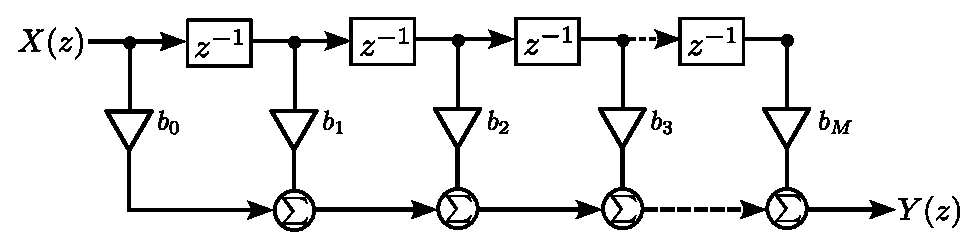
\includegraphics[width=.8\textwidth]{images/FIR_filter.eps}
    \caption{Direct form of a finite impulse response (FIR) filter with linear phase}
    \label{fig:FIR}
\end{figure}


Taking the inverse $z$-transform, we get
\[
    Y(z) = X(z) \underbrace{\sum_{k=0}^{M} b_k \cdot z^{-k}}_{H(z)} \quad \xrightarrow{\mathcal{Z}^{-1}} \quad
    y[n] = \sum_{k=0}^{M} b_k \cdot x[n-k].
\]

\paragraph{Properties of FIR filters}
\begin{itemize}
    \item No poles: all-zero filters. The system function $H(z)$ is defined for the entire $z$-plane.
    \item They are inherently stable. Stability of an LTI system:
    \[
        \sum_{n=-\infty}^{+\infty} \lvert h[n] \rvert < \infty
    \]
    with $h[n]$ of finite length. This condition is always satisfied.
\end{itemize}

\subsubsection{FIR Filter Design by Truncation}
Truncation of the impulse response is a simple way to design FIR filters. Mathematically, we multiply the impulse response with a \textit{window function}.

\begin{ex}{}
The impulse response of an ideal low-pass filter (\autoref{fig:ir_low_pass}) is 
\[
    H(e^{j\omega}) = 
    \begin{cases} 
    1, & \text{if} \ \lvert \omega \rvert \leq \omega_{c} \\ 
    0, & \text{otherwise}
    \end{cases}
    \quad \to \quad
    h_{d}[n] = \frac{\omega_{c}}{\pi}\frac{\sin\omega_{c}n}{\omega_{c}n}
\]
\begin{figure}[H]
    \centering
    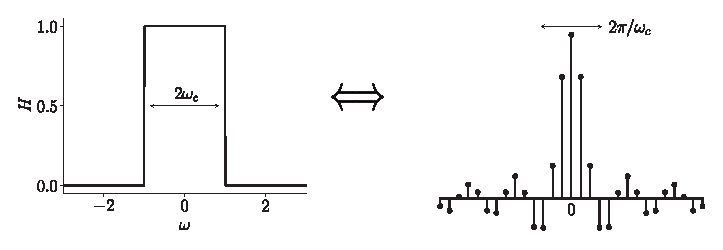
\includegraphics{images/low-pass-response.eps}
    \caption{Impulse response of an ideal low-pass filter}
    \label{fig:ir_low_pass}
\end{figure}

The FIR filter $h[n]$ is created by windowing the ideal response:
\[
    h_{T}[n] = h[n] w[n], \quad \text{for} \ n=0, 1, ..., M
\]
where $w[n]$ is the window function that is only non-zero for $n=0, 1, ..., M$. \autoref{fig:windowing} illustrates the truncation process with a rectangular window function.

\begin{figure}[H]
    \centering
    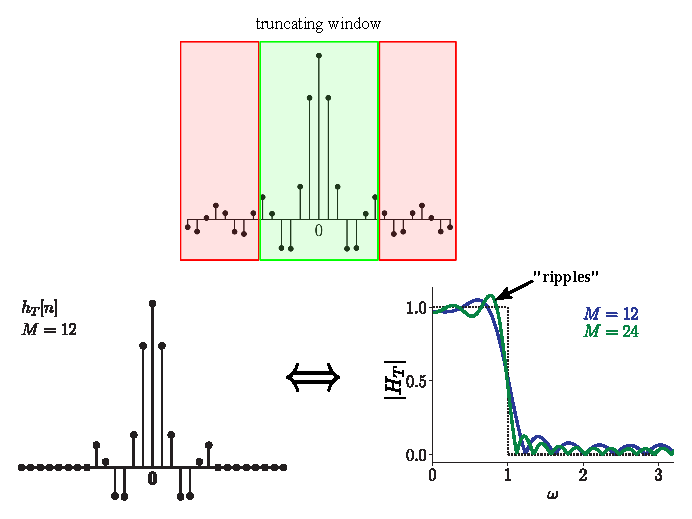
\includegraphics{images/windowing.eps}
    \caption{Truncation of $h[n]$ with a rectangular window.}
    \label{fig:windowing}
\end{figure}

\paragraph{Remarks}
\begin{enumerate}
    \item Typically, the impulse response $h[n]$ is  \textit{non-causal} or at least \textit{non-FIR}. The signal illustrated above is both non-causal and infinite.

    \item Truncation of $h[n]$ to $\pm \frac{M}{2}$ makes the signal finite. Furthermore, the signal will become causal if we delay the truncated signal $h_T[n]$ by $M/2$.

    \item The ripples (indicated with an arrow in \autoref{fig:windowing}) are produced due to the discontinuity of the window \footnote{This can be derived by quantifying the mean squared error in the frequency domain between $H(e^{j\omega})$ and $H_T(e^{j\omega})$. Clearly, the MSE is minimised when $h[n]=h_T[n]$, but practically not possible (regardless of the number of $M$ used in truncation)!}, also referred to as the ``Gibbs phenomenon". 
\end{enumerate}
\end{ex}
From remark (3), although it is impossible to fully remove the ripples, it is possible to truncate with other windows to reduce the ripples. \textit{Hanning}, \textit{Hamming}, \textit{Blackman} (also referred to as \textit{Blackman-Harris}) are examples of alternative windows to rectangular window.

\subsubsection{FIR Filter Design by Other Methods}
\textit{This section is NOT covered in the lectures. Massive materials are adopted from textbooks. Please take prudence with the notations used in this section.}
\begin{itemize}
    \item Frequency sampling: take the IDFT of $M+1$ equally spaced samples of $H(e^{j\omega})$.
    \[
    H_{FIR}(e^{j\omega})=\sum_{n=0}^{M} h[n]e^{-j\omega n} \bigg\lvert_{\omega = \frac{2\pi}{M}k, \quad k=0, 1, 2..., M} \quad \xrightarrow{\mathcal{F}^{-1}} h_{FIR}[n]
    \]
        \begin{itemize}
            \item Pros: giving an exact match at the sample points.
            \item Cons: intermediate approximation is poor if the spectrum varies rapidly.
        \end{itemize}
    \item Least-square
    \item Equiripple method: find the FIR filter to minimise the \textit{maximum weighted error}, $\mathcal{E}$, between the desired response and the actual frequency response of an FIR filter.
    \[
    \mathcal{E}(e^{j\omega}) = \mathcal{W}(\omega)  \lvert H(e^{j\omega}) - H_{FIR}(e^{j\omega})  \rvert
    \]
    where $\mathcal{W}(\omega)$ is a weighting function used to adjust the weightings applied to the pass band, transition band, and stopband:
    \[
    \mathcal{W}(\omega) = \begin{cases}
        1/\delta_1, & 0 \leq \omega \leq \omega_c\\
        0, & \omega_c < \omega < \omega_{s}\\
        1/\delta_2, & \omega_{s} \leq \omega \leq \pi\\
    \end{cases}
    \]
\end{itemize}


\subsection{Infinite Impulse Response (IIR) Filters}

\subsubsection{Definition}
If $N \neq 0$ in the generalized difference equation, the system function carries a recursive part in the denominator. 
\[
    H(z) = \frac{\sum_{k=0}^{M} b_{k} \cdot z^{-k}}{1 - \sum_{k=1}^{N} a_{k} \cdot z^{-k}} \quad \xrightarrow{\mathcal{Z}^{-1}} \quad y[n] = \sum_{k=0}^{M}b_{k} \cdot x[n-k] - \sum_{k=0}^{N}a_{k} \cdot y[n-k] 
\]

\begin{figure}[H]
    \centering
    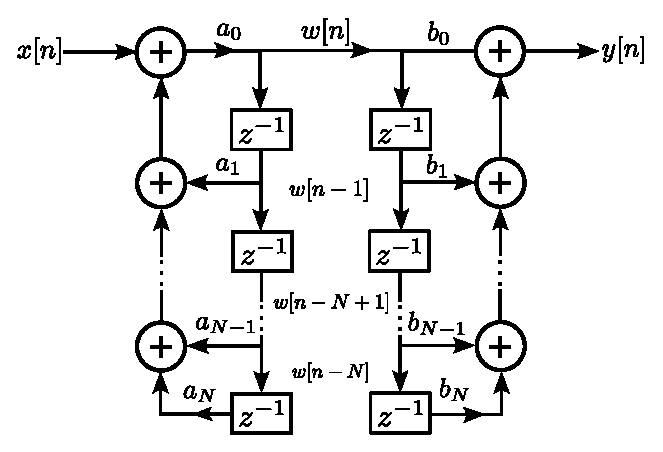
\includegraphics{images/IIR_filter.eps}
    \caption{Direct realisation of a digital IIR filter}
    \label{fig:IIR_direct}
\end{figure}

% Consider the following impulse response:
% \[
%     h[n] = b_0 a^{n} u[n] + b_1 a^{n-1} u[n-1]
% \]
% This is an infinite-length sequence, the filter is an infinite response filter. The system function thus
% \[
%     H(z) = \frac{b_0 + b_1 z^{-1}}{1 - az^{-1}}, \quad \lvert z \rvert > \lvert a \rvert
% \]
% Therefore, the system can also be seen as derived by the following difference equation:
% \[
%     y[n] - ay[n-1] = b_0 x[n] + b_1x[n-1]
% \]

% Structure for IIR filters
% \[
%     y[n] = \sum_{k=1}^{N} a_{k}y[n-k] + \sum_{k=0}^{M} b_{k}x[n-k]
% \]
% The general form for the system function is
% \[
%     H(z) = \frac{\sum_{k=0}^{M} b_{k} z^{-k}}{1 - \sum_{k=1}^{N} a_{k}z^{-k}}
% \]
% The output of the system in the $z$-domain is obtained as
% \[
%     Y(z) = H(z)X(z)
% \]
% or
% \[
%     Y(z) = \sum_{k=0}^{M} b_{k} b_{k} z^{-k} W(z), \quad \text{with} \quad W(z) = \frac{1}{1-\sum_{k=1}^{N} a_{k}z^{-k}}X(z)
% \]
The system function $H(z)$ can also be represented as a cascade of filters by factorizing the numerator and denominator:
\[
    H(z) = A \frac{\Pi_{k=1}^{M_1}(1-f_{k}z^{-1}) \Pi_{k=1}^{M_2}(1-g_{k}z^{-1})(1-g_{k}^{*}z^{-1})}{\Pi_{k=1}^{N_1}(1-c_{k}z^{-1}) \Pi_{k=1}^{N_2}(1-d_{k}z^{-1})(1-d_{k}^{*}z^{-1})}
\]


\subsubsection{IIR Filter Design by Bilinear Transformation}
The bilinear transformation transforms from the continuous-time systems in the Laplace domain to discrete-time systems in the $z$-domain. \\

An \textit{analogue} filter can always be described by a frequency domain system function of the general form, 
\[
    H(s) = \alpha\frac{(s-z_{1})(s-z_{2})...(s-z_{m})}{(s-p_{1})(s-p_{2})...(s-p_{n})}
\]
In bilinear transformation, we replace $s$ by $z$:
\[
    z = \frac{\alpha+s}{\alpha-s} \Leftrightarrow s 
    = \alpha \frac{z-1}{z+1} \bigg \lvert_{z=e^{j\omega}} 
    = \alpha \frac{e^{j\frac{\omega}{2}} - e^{-j\frac{\omega}{2}}}{e^{j\frac{\omega}{2}} + e^{-j\frac{\omega}{2}}} 
    = j\alpha\tan\frac{\omega}{2} = j\Omega
\]
Frequency mapping:
\[
    \Omega = \alpha \tan\frac{\omega}{2}
\]
Overall, the bilinear transformation allows the design of IIR filters from analogue filters: $H(s) \to H(\omega)$.